\documentclass[aspectratio=169]{beamer}
\usepackage{pgf}
\usepackage{multimedia}
\usepackage{colortbl,tabularx,mathrsfs,calligra,xcolor}
\usepackage{amsmath,amsfonts,amssymb,amsthm}
\usepackage{ragged2e}
\usepackage{setspace}
\usepackage{filecontents}
\usepackage{caption}
\usepackage{subcaption}
\usepackage{contour}
\usepackage{fancybox}
\usepackage{wrapfig}
\usepackage{multirow}
\usepackage{multicol}
\usepackage{pgfplots, tkz-euclide,calc}
    \usetikzlibrary{patterns,snakes,shapes.arrows,shapes.geometric,arrows}
\usepackage{listings}
\usepackage{enumitem}
\usepackage{pifont}
\usepackage[scaled]{berasans}
    \renewcommand*\familydefault{\sfdefault}  %% Only if the base font of the document is to be sans serif
\usepackage[T1]{fontenc}
\usepackage{hyperref}
\hypersetup{
    filecolor=magenta,      
    urlcolor=cyan,
    pdftitle={Overleaf Example},
    pdfpagemode=FullScreen,
    }
\renewcommand*\familydefault{\sfdefault} %% Only if the base font of the document is to be sans serif

\graphicspath{{C:/Users/teoso/OneDrive/Documents/Asisten Dosen & Lab/Asisten Laboratorium/Alpro 1/PPT/Graphicx/}}

\definecolor{HIMAmuda}{HTML}{01D1FD}
\definecolor{HIMAtua}{HTML}{02016A}
\definecolor{HIMAabu}{HTML}{CBCBCC}
\definecolor{PastelGreen}{HTML}{77DD77}
\definecolor{pgray}{rgb}{0.5,0.5,0.5}
\definecolor{pblue}{rgb}{0.13,0.13,1}
\definecolor{pgreen}{rgb}{0,0.5,0}
\definecolor{pred}{rgb}{0.9,0,0}
\definecolor{pgrey}{rgb}{0.46,0.45,0.48}
\definecolor{pcyan}{HTML}{D4EFFC}
\definecolor{lblue}{HTML}{00AEEF}
\definecolor{input}{HTML}{AAE1FA}
\definecolor{bg}{rgb}{0.95, 0.95, 0.92}
\definecolor{vscode}{HTML}{282A36}

\usetheme{Madrid}

\setbeamercolor{palette primary}{bg=HIMAtua,fg=white}
\setbeamercolor{palette secondary}{bg=HIMAmuda,fg=black}
\setbeamercolor{palette tertiary}{bg=HIMAabu,fg=black}
\setbeamercolor{palette quaternary}{bg=HIMAmuda,fg=white}
\setbeamercolor{structure}{fg=HIMAmuda} % itemize, enumerate, etc
\setbeamercolor{section in toc}{fg=HIMAtua} % TOC sections
\setbeamercolor{block title alerted}{fg=white,bg=magenta}
\setbeamercolor{block body alerted}{fg=black!90,bg=pink}

\usefonttheme{professionalfonts}
\setbeamertemplate{theorems}[numbered]
\setbeamertemplate{itemize items}[circle]

\usebackgroundtemplate{%
\tikz[overlay,remember picture] \node[opacity=0.1, at=(current page.center)]{\includegraphics[width=\paperwidth]{plana class}};
}

\renewcommand\thesubfigure{\arabic{subfigure}}
\newtheorem*{funfact}{Fun Fact}
\newtheorem{latihan}{Latihan}
\newtheorem*{definisi}{Definisi}
\newtheorem{teorema}{Teorema}
\theoremstyle{definition}
\newtheorem*{contoh}{Contoh}
\newtheorem*{masalah}{Masalah}
\newcommand{\R}{\mathbb{R}}

\AtBeginEnvironment{funfact}{%
  \setbeamercolor{block title}{fg=white,bg=PastelGreen} % Set title background to pastel green and text to white
  \setbeamercolor{block body}{parent=normal text,bg=PastelGreen!30!white} % Set body background to a lighter pastel green
}
\AtBeginEnvironment{definisi}{
    \setbeamercolor{block title}{fg=white,bg=HIMAtua}
    \setbeamercolor{block body}{parent=normal text,bg=HIMAtua!30!white}
}
\AtBeginEnvironment{teorema}{
    \setbeamercolor{block title}{bg=darkgray,fg=white}
    \setbeamercolor{block body}{parent=pallette tertiary,bg=HIMAabu!30!white}
}
\AtBeginEnvironment{latihan}{%
  \setbeamercolor{block title}{fg=white,bg=PastelGreen} % Set title background to pastel green and text to white
  \setbeamercolor{block body}{parent=normal text,bg=PastelGreen!30!white} % Set body background to a lighter pastel green
}
\AtBeginEnvironment{masalah}{%
  \setbeamercolor{block title}{fg=white,bg=teal} % Set title background to pastel green and text to white
  \setbeamercolor{block body}{parent=normal text,bg=teal!30!white} % Set body background to a lighter pastel green
}

\renewcommand{\arraystretch}{1.3}

\usepackage{listings}

\lstdefinestyle{standard}{
    language            = Java,
    showspaces          = false,
    showtabs            = false,
    breaklines          = true,
    showstringspaces    = false,
    breakatwhitespace   = true,
    commentstyle        = \color{pgray},
    keywordstyle        = \color{pblue},
    stringstyle         = \color{pgreen},
    basicstyle          = \footnotesize\ttfamily,
    frame               = single,
    backgroundcolor     = \color{brown!10!white},
    escapeinside        = {(*}{*)},
    numbers             = left, % {none, left, right}
    numberstyle         = \scriptsize\color{lightgray},
    numbersep           = -8pt,
    }

\lstdefinestyle{output}{
    language=Java,
    backgroundcolor     =\color{vscode},
    basicstyle          =\footnotesize\ttfamily\color{white},
    frame               =shadowbox,
    escapeinside        ={(*}{*)},
    showspaces          =false,
    showtabs            =false,
    breaklines          =true,
    showstringspaces    =false,
    breakatwhitespace   =true,
    rulesepcolor        =\color{HIMAtua!50!white},
    rulecolor           =\color{HIMAtua!50!white},
    numbers             =none,
    }

\lstset{style=standard}

\tikzstyle{startstop} = [rectangle, rounded corners, 
minimum width=2cm, 
minimum height=1cm,
text centered, 
draw=black, 
fill=pink]

\tikzstyle{io} = [trapezium, 
trapezium stretches=true, % A later addition
trapezium left angle=70, 
trapezium right angle=110, 
minimum width=2cm, 
minimum height=1cm, text centered, 
draw=black, fill=HIMAmuda]

\tikzstyle{process} = [rectangle, 
minimum width=2cm, 
minimum height=1cm, 
text centered, 
text width=1cm, 
draw=black, 
fill=HIMAabu]

\tikzstyle{decision} = [diamond, 
minimum width=2cm, 
minimum height=1cm, 
text centered, 
draw=black, 
fill=PastelGreen]
\tikzstyle{arrow} = [thick,->,>=stealth]

\newcommand{\enter}{\raisebox{-1.8pt}{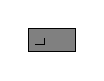
\begin{tikzpicture}[scale=0.3]
    \draw[thin,fill=gray] (0,0) rectangle (2,1);
    \draw (0.3,0.3) -- (0.7,0.3)--(0.7,0.6);     
\end{tikzpicture}}}

\newcommand{\inputscan}[1]{\raisebox{0pt}[1pt]{\colorbox{darkgray}{#1}}}

\author[Tew \& Haf]{Hafidz Mulia\\Teosofi Hidayah Agung}
\date{30 September 2024}
\title[Alpro 1 - Week 4]{Struktur Kontrol}
\institute[Matematika ITS]{Departemen Matematika\\ Institut Teknologi Sepuluh Nopember}
\titlegraphic{{\includegraphics[scale=0.02]{M.png}$\quad$\includegraphics[scale=0.2]{Provicom.png}}}

\begin{document}
    {\usebackgroundtemplate{
        \tikz[overlay,remember picture] \node[opacity=0.2, at=(current page.center)]{\includegraphics[width=\paperwidth]{bg_2}};}
    \begin{frame}
        \titlepage
    \end{frame}
    }

    \AtBeginSection{
    {\usebackgroundtemplate{
     \tikz[overlay,remember picture] \node[opacity=0.1, at=(current page.center)]{\includegraphics[width=\paperwidth]{Java code}};}
    \begin{frame}{Daftar isi}
        \tableofcontents[currentsection]
    \end{frame}}
    }
    {\usebackgroundtemplate{
        \tikz[overlay,remember picture] \node[opacity=0.1, at=(current page.center)]{\includegraphics[width=\paperwidth]{choice}};}
    \begin{frame}
        \begin{masalah}
            Kata "Jika", "Andaikan", dan "Misalnya" merupakan kata yang sering kita gunakan untuk memikirkan akibat dari suatu keputusan. Namun percayalah bahwa akibat yang kita dapatkan tergantung pada kondisi yang kita pilih.\\
            \vspace*{0.2cm}
            Dari sinilah muncul sebuah mekanisme dalam bahasa pemrograman yang berguna untuk menjalankan suatu perintah berdasarkan kondisi tertentu. 
        \end{masalah}
        \begin{exampleblock}{}
            \begin{quote}
                "Kegagalan bukanlah pilihan" -- Alucard
            \end{quote}
        \end{exampleblock}
    \end{frame}
    }
    
    \section{If-Else}
    \begin{frame}[fragile]
        \frametitle{\insertsection}
        \begin{definisi}
            If-else merupakan struktur kontrol yang digunakan untuk menjalankan suatu perintah jika kondisi yang diberikan bernilai benar. Jika kondisi bernilai salah, maka perintah lain yang akan dijalankan.
        \end{definisi}
        \begin{lstlisting}[numbers=none]
    if (kondisi 1) {
        // Perintah yang dijalankan jika kondisi 1 benar
    }
    else if (kondisi 2) {
        // Perintah yang dijalankan jika kondisi 2 benar
    }
    (*\ldots*)
    (*\ldots*)
    else {
        // Perintah yang dijalankan jika semua kondisi diatas salah
    }
        \end{lstlisting}
    \end{frame}

    \begin{frame}
        \frametitle{\insertsection}
        \begin{figure}
            \centering
            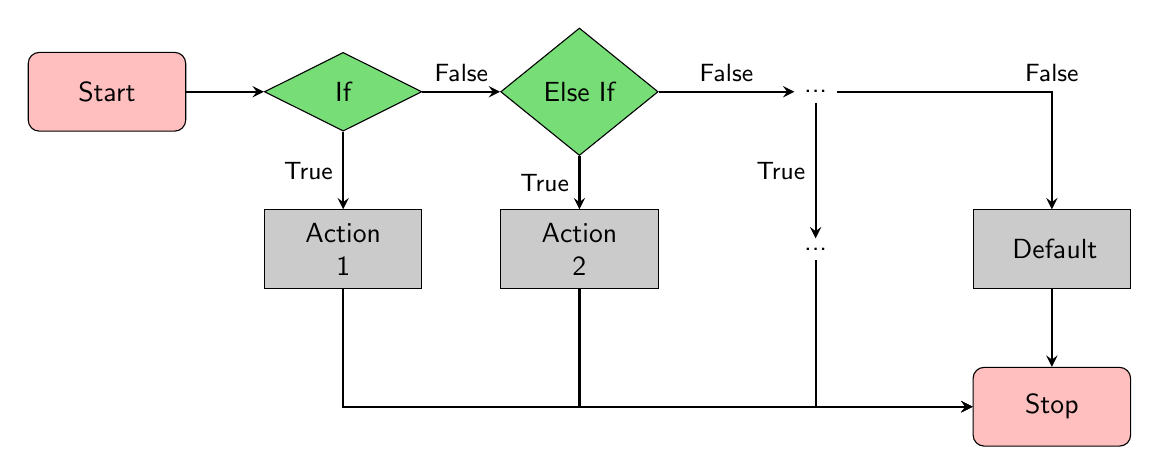
\begin{tikzpicture}[scale=0.5]
                \node (start) [startstop] {Start};
                \node (kondisi1) [decision, right of=start, xshift=2cm] {If};
                \node (kondisi2) [decision, right of=kondisi1, xshift=2cm] {Else If};
                \node (kondisiN) [right of=kondisi2, xshift=2cm]{...};
                \node (action1) [process, below of=kondisi1, yshift=-1cm] {Action 1};
                \node (action2) [process, below of=kondisi2, yshift=-1cm] {Action 2};
                \node (actionN) [below of=kondisiN, yshift=-1cm] {...};
                \node (default) [process, below of=kondisiN, yshift=-1cm, xshift=3cm] {Default};
                \node (stop) [startstop, below of=default, yshift=-1cm] {Stop};

                \draw [arrow] (start) -- (kondisi1);
                \draw [arrow] (kondisi1) -- node[anchor=east] {\small True} (action1);
                \draw [arrow] (kondisi1) -- node[anchor=south] {\small False} (kondisi2);
                \draw [arrow] (kondisi2) -- node[anchor=east] {\small True} (action2);
                \draw [arrow] (kondisi2) -- node[anchor=south] {\small False} (kondisiN);
                \draw [arrow] (kondisiN) -- node[anchor=east] {\small True} (actionN);
                \draw [arrow] (kondisiN) -| node[anchor=south] {\small False} (default);
                \draw [arrow] (action1) |- (stop);
                \draw [arrow] (action2) |- (stop);
                \draw [arrow] (actionN) |- (stop);
                \draw [arrow] (default) -- (stop);
            \end{tikzpicture}
            \caption{Flowchart If-Else}
        \end{figure}
    \end{frame}

    \begin{frame}[fragile]
        \frametitle{\insertsection}
        \begin{lstlisting}[caption={Contoh If-Else}, firstnumber=5]
    int number = 10;

    if (number > 0) {
        System.out.println("Angka positif");
    } else if (number < 0) {
        System.out.println("Angka negatif");
    } else {
        System.out.println("Angka nol");
    }
        \end{lstlisting}
    \end{frame}

    \begin{frame}[fragile]
        \frametitle{\insertsection}
        \begin{block}{Nested If-Else}
            Nested berarti bersarang. Nested If-Else merupakan struktur kontrol If-Else yang diletakkan di dalam If-Else lainnya.
        \end{block}
        \begin{lstlisting}[firstnumber=23,caption={Contoh Nested If-Else}]
    if (kondisi 1) {
        if (kondisi 2) {
        // Dijalankan jika kondisi 1 dan kondisi 2 benar
        } else {
        // Dijalankan jika kondisi 1 benar namun kondisi 2 salah
        }
    } else {
        // Dijalankan jika kondisi 1 salah
    }
        \end{lstlisting}
    \end{frame}

    \section{Switch}
    \begin{frame}
        \frametitle{\insertsection}
        \begin{definisi}
            Switch merupakan struktur kontrol yang digunakan untuk memilih satu dari beberapa pilihan yang ada. Pilihan tersebut berdasarkan nilai dari ekspresi yang diberikan. 
        \end{definisi}
        \begin{alertblock}{Catatan}
            Switch hanya dapat digunakan untuk tipe data primitif seperti int, char, dll.
        \end{alertblock}
    \end{frame}

    \begin{frame}[fragile]
        \frametitle{\insertsection}
        \begin{lstlisting}[firstnumber=4,caption={Struktur Switch}]
    switch (variabel) {
        case nilai_1:
            // Perintah yang dijalankan jika variabel = nilai_1
            break;
        case nilai_2:
            // Perintah yang dijalankan jika variabel = nilai_2
            break;
        (*\ldots*)
        (*\ldots*)
        default:
            // Perintah yang dijalankan jika tidak ada nilai yang cocok
    }
        \end{lstlisting}
    \end{frame}

    \begin{frame}[fragile]
        \frametitle{\insertsection}
        \begin{alertblock}{Perhatikan}
            Jika tidak ada \texttt{break} setelah setiap \texttt{case}, maka semua perintah setelah \texttt{case} yang cocok akan dijalankan bahkan untuk \texttt{default}. 
        \end{alertblock}
        \begin{lstlisting}[firstnumber=9]
    switch (number) {
        case 1:
            System.out.println("Satu");
        case 2:
            System.out.println("Dua");
        default:
            System.out.println("Bukan satu atau dua");
    }
        \end{lstlisting}
    \end{frame}

    \begin{frame}[fragile]
        \frametitle{\insertsection}
        \begin{lstlisting}[style=output, caption={Contoh Output}]
    number = (*\inputscan{2} \enter*);
    Dua
    Bukan satu atau dua
        \end{lstlisting}
        \begin{lstlisting}[style=output]
    number = (*\inputscan{1} \enter*);
    Satu
    Dua
    Bukan satu atau dua
        \end{lstlisting}
    \end{frame}

    \section{Ternary Operator}
    \begin{frame}[fragile]
        \frametitle{\insertsection}
        \begin{definisi}
            Ternary Operator merupakan operator yang digunakan untuk menggantikan struktur If-Else yang sederhana. Ternary Operator terdiri dari tiga bagian, yaitu kondisi, nilai jika benar, dan nilai jika salah.
        \end{definisi}
        \begin{lstlisting}[numbers=none]
    variabel = ekspresi_logika ? nilai_jika_benar : nilai_jika_salah;
        \end{lstlisting}
        \begin{lstlisting}[caption={Contoh Ternary Operator}, firstnumber=34]
    Scanner input = new Scanner(System.in);
    int number = input.nextInt();
    System.out.println(number > 0 ? "Positif" : "Negatif");
        \end{lstlisting}
    \end{frame}

    \section{Latihan}
    \begin{frame}
        \begin{latihan}
            Buatlah program yang menerima inputan berupa nilai mahasiswa. Kemudian program akan menampilkan keterangan nilai berdasarkan rentang nilai berikut:
            \begin{table}
                \centering
                \begin{tabular}{|c|c|}
                    \hline
                    Rentang Nilai & Keterangan \\
                    \hline
                    86 - 100 & A \\
                    76 - 85 & AB \\
                    66 - 75 & B \\
                    61 - 65 & BC \\
                    56 - 60 & C \\
                    41 - 55 & D \\
                    0 - 40 & E \\
                    \hline
                \end{tabular}
            \end{table} 
        \end{latihan}
    \end{frame}

    \begin{frame}
        \begin{latihan}
            Buatlah program yang menampilkan hari "Minggu", "Senin", "Selasa", "Rabu", "Kamis", "Jumat", dan "Sabtu", jika nilai dari variabel hari masing-masing adalah 0, 1, 2, 3, 4, 5, 6.
        \end{latihan}
        \begin{latihan}
            Buatlah program yang menerima inputan berupa bilangan bulat. Program akan menampilkan beberapa hal berikut:
            \begin{itemize}[label=$\bullet$]
                \item Bilangan ganjil atau genap
                \item Bilangan positif atau negatif
                \item Bilangan kuadrat sempurna atau bukan 
            \end{itemize}
        \end{latihan}
    \end{frame}
\end{document}